\section{Desenho da Pesquisa}
\label{desenhodepesquisa}

Segundo \citeauthor{marconi2003} (\citeyear{marconi2003}), o desenvolvimento de um projeto de pesquisa compreende seis passos: 
“Seleção do tópico ou problema para a investigação, definição e diferenciação do problema, levantamento de hipóteses de trabalho, coleta, sistematização e classificação dos dados, análise e interpretação dos dados e relatório do resultado da pesquisa”.

Esses passos podem ser agrupados em quatro fases: preparação de pesquisa, fases da pesquisa, execução da pesquisa e relatório de pesquisa. A preparação de pesquisa será desconsiderada aqui, por envolver escolha do tema, constituição de equipe de trabalho, cronograma e outros. \cite{marconi2003}


Na etapa de Fases da pesquisa, serão tratados: a escolha do problema que será investigado, a definição deste, e o levantamento das hipóteses acerca do problema. Essa etapa irá envolver:
\begin{itemize}
    \item \textbf{Revisão rápida de literatura}: visa observar o atual panorama da inovação social aberta praticada pelas universidades em instituições do terceiro setor nas principais bases de dados da área da ciência da computação, através da metodologia de revisão rápida proposta por \citeauthor{cartaxo2020} (\citeyear{cartaxo2020});
    \item \textbf{Identificação dos principais atores:} como a inovação social aberta envolve diferentes instituições, e por consequência, uma gama de diferentes atores, deverão ser identificados quais os principais que deverão ser observados com uma maior atenção, e que poderão proporcionar \textit{feedbacks} posteriores a equipe de pesquisa sobre os métodos propostos.
    \item \textbf{Criação do protocolo de entrevistas, grupos focais e formulários}: para colher os \textit{feedbacks} dos principais atores envolvidos, serão criadas estratégias de entrevistas, grupos focais e formulários com os participantes. Essas entrevistas deverão ser validadas anteriormente pela equipe de pesquisa, antes de serem aplicadas.
\end{itemize}

Na etapa de Execução da pesquisa será realizada a coleta e análise de dados, a criação do processo e validação, que envolverá: 
\begin{itemize}
    \item \textbf{Realização das entrevistas, grupos focais e formulários:} realização do que foi concebido na etapa anterior;
    \item \textbf{Análise das entrevistas, grupos focais e formulários}: serão analisadas as entrevistas, grupos focais e formulários, além de todas as questões colocadas pelos entrevistados;
    \item \textbf{Criação do processo para projeto de extensão}: a criação do projeto de Extensão utilizando a Inovação Social Aberta no terceiro setor, após observar os \textit{feedbacks} colhidos nas entrevistas;
    \item \textbf{Validação do processo para projeto de extensão}: o processo proposto será validado durante sua execução, e os \textit{feedbacks} serão coletados durante a análise de dados, que podem ocorrer diversas vezes.
\end{itemize}

A etapa de Relatório de pesquisa trará os resultados obtidos através da pesquisa, suas conclusões e metodologia utilizada. Essa última etapa é a publicização do que foi realizado em toda a pesquisa, e consiste em:
\begin{itemize}
    \item \textbf{Sintetização dos resultados obtidos}: A exposição de todo o conhecimento obtido com os dados trabalhados durante a pesquisa;
    \item \textbf{Confecção da Dissertação}: Escrita da dissertação de mestrado;
    \item \textbf{Apresentação do trabalho}: Apresentar uma sumarização de toda a pesquisa para a banca;
    \item \textbf{Correções finais}: realizar correções na dissertação conforme as orientações da banca.
\end{itemize}

A pesquisa será realizada em ciclos iterativos, visando o incremento das sugestões de melhorias propostas pelos \textit{stakeholders} no processo ao longo da sua execução. Por conta disso, algumas etapas serão provavelmente realizadas mais de uma vez. Esses passos são necessários para garantir o procedimento e o tratamento científico exigido pelo trabalho. Para facilitar a compreensão da forma como a pesquisa se desenvolverá, a figura abaixo traz uma síntese do desenho da pesquisa:

\begin{figure}[H]
    \caption{Desenho de pesquisa proposto}
    \centering
    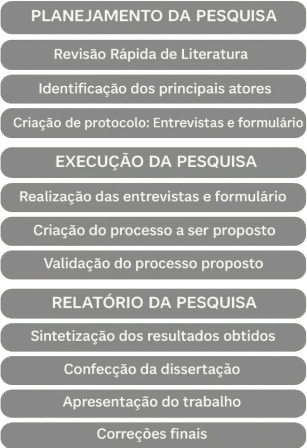
\includegraphics[width=0.6\linewidth]{images/metodologia/desenhodepesquisa.png}
    \label{fig:desenhodepesquisa}
    \vspace{0.2cm}

{\centering Fonte: O autor (2024), baseado em Marconi e Lakatos (2003). \par}
\end{figure}

